Measurements used an AMD Ryzen 9 7950X CPU, eight OpenBLAS threads,
Python 3.10.12, NumPy 1.24.3 and OpenBLAS 0.3.21. Batch size was 128.
No GPU was used. Each reported prediction time is one wall-clock
measurement after a short warm-up, not an average of repeated runs.
Timings depend on the machine and its concurrent workload.

The common comparison sample contained one test image per class, selected
with \code{default\_rng} and seed 2026: 100 images in total. Every classifier
used all 50,000 training examples. Each optimized model agreed with its
original on \textbf{all 100 predictions}. This validates the sample, not
every possible numerical tie. The original NCC was also run on the entire
test set, yielding agreement on all 10,000 predictions.

\begin{table}[t]
\caption{Full evaluation on 10,000 test images}
\label{tab:accuracy}
\centering\small
\begin{tabular}{@{}lrr@{}}
\toprule
Classifier & Correct predictions & Accuracy\\
\midrule
1-NN & 1\,755 & 17.55\%\\
3-NN & 1\,748 & 17.48\%\\
NCC & 1\,004 & 10.04\%\\
\bottomrule
\end{tabular}
\end{table}

\begin{figure}[t]
\centering
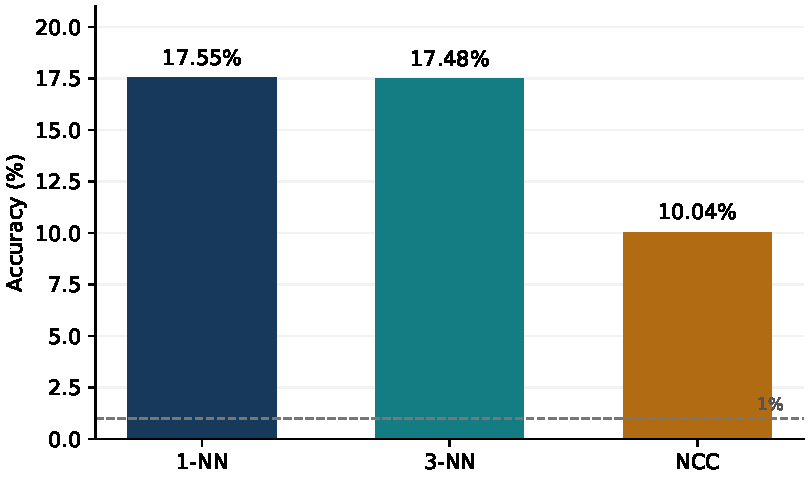
\includegraphics[width=\columnwidth]{figures/accuracy.pdf}
\caption{Measured accuracy of the optimized implementations on the full
test set. The dashed line marks the 1\% achieved by a constant class
prediction on this balanced dataset.}
\label{fig:accuracy}
\end{figure}

\begin{table}[t]
\caption{Prediction time on the same 100-image sample}
\label{tab:timing}
\centering\small
\begin{tabular}{@{}lrrr@{}}
\toprule
Model & Original (s) & Optimized (s) & Speedup\\
\midrule
1-NN & 24.173 & 0.0916 & $263.8\times$\\
3-NN & 24.031 & 0.1095 & $219.5\times$\\
NCC & 0.0417 & 0.000589 & $70.9\times$\\
\bottomrule
\end{tabular}
\end{table}

Table~\ref{tab:timing} uses separate prediction calls for each classifier.
In the final full run, the shared 1-NN/3-NN search took
\textbf{10.319 s} for all 10,000 images. This is the time for
\emph{both results together}, not an independent runtime for each model.
It includes neighbor selection, voting and progress messages.
Optimized NCC prediction took 0.0567 s; the original NCC took 4.158 s
on the same full set.

The original k-NN \code{fit()} only stores a dictionary reference and
was measured at approximately $1\,\mu$s. Shared optimized k-NN preparation
took 1.523 s because it constructs a contiguous \code{float64} matrix,
labels and squared norms. This preparation is paid once and excludes
loading and grouping. NCC centroid construction took about 0.023 s
in both versions.

The original k-NN implementations were not run on the entire test set.
Extrapolating their sample timings suggests about 40 minutes per original
pass; this is an \emph{estimate}, not a measured full run. The original
implementation is functional. The observed CPU acceleration made GPU
support and PCA unnecessary for this experiment.

The files \code{results/cpu\_benchmark.json} and
\code{results/predictions.npz} retain the settings, measurements and full
predictions in original test-set order. The JSON also records sample
indices and SHA-256 hashes of the measured source files.
